\documentclass[10pt,twoside,english,a4paper]{article}
%I can write this in English
% Engineering methods

\usepackage{graphicx} % Required for inserting images

%\usepackage[T1]{fontenc}
\usepackage[IL2]{fontenc} % lepšia sadzba písmena Ľ než v T1
\usepackage[utf8]{inputenc}
\usepackage{url} % príkaz \url na formátovanie URL
\usepackage{hyperref} % odkazy v texte budú aktívne (pri niektorých triedach dokumentov spôsobuje posun textu)

\usepackage{cite}
\graphicspath{{images/}}
%\usepackage{times}

\pagestyle{headings}

\title{Delivering Relevant Product Recommendations in Finance\thanks{Semester project from subject Engineering methods, academic year 2024/25, management: Martin Sabo}} % 

\author{Mykhailo Chepara\\[2pt]
	{\small Slovak Technical University in Bratislava}\\
	{\small Faculty of Information and Information Technologies}\\
	{\small \texttt{xchepara@stuba.sk}}
	}

\date{\small October 1 2024} % upravte



\begin{document}


\maketitle


\begin{abstract}
To begin with why is that topic? 
One of my friends is working in a financing company, therefore I'm genuinely curious how does a bank recommend products to it's customers. It's a useful tool for a bank to increase it's revenue but can it be enhanced? And if yes then how?

Now to the points that I'm going to untangle in this article:
\begin{itemize}
    \item What's a recommendation system
    \begin{itemize}
        \item Types of recommendation systems
    \end{itemize}
    
    \item How does a recommendation system in a bank work
    \begin{itemize} 
             \item It's structure: ways of utilizing data
             \item Algorithms
             \item Which data types are used
    \end{itemize}
    
    \item Time it takes to learn and to be able to recommend something
    \begin{itemize}
        \item When it learns the most efficiently and can you increase speed of learning
    \end{itemize}
    
    \item Issues with system
    \begin{itemize}
        \item Lack of data
        \item New item introduction
        \item Disability to recommend anything relevant to a user
    \end{itemize}
    
    \item Enhancement of the system
    \begin{itemize}
        \item Merging the system with another system in order to increase it's efficiency and accuracy
        \item Which systems can be fused with recommendation system
        \item Can something new be embedded into it
        \item What can be embedded
    
    \end{itemize}
    

\end{itemize}

sources - https://kanini.com/blog/banking-recommendation-system-use-cases/

\end{abstract}


\tableofcontents

\section{Recommendation system}

\subsection{Definition of a recommendation system}
Recommendation system is an algorithm which is trained on huge amounts of data in order to mimic or predict next purchases of the customer on whom data it was trained on.
In a nutshell it takes one record of data per time and iterates with it to specify parameters and refine them, it does it with each and every record by that becoming more accurate.

So it's a system designed for each and every customer individually

\subsection{Variations of recommendation systems}


\section{Structures and principles of workflow}

\subsection{Structure}
Blah blah blah...
\begin{center}

%\begin{{figure}[h!]

%\caption{Structure of the system}
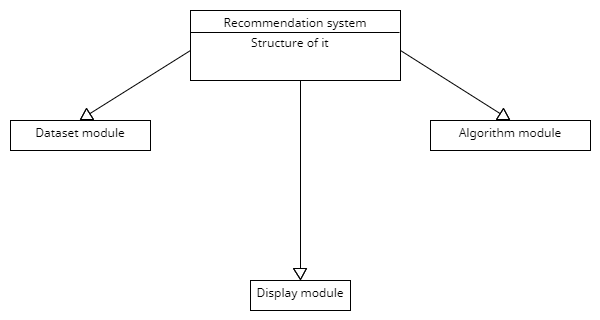
\includegraphics[width=0.8\textwidth]{system_structure}
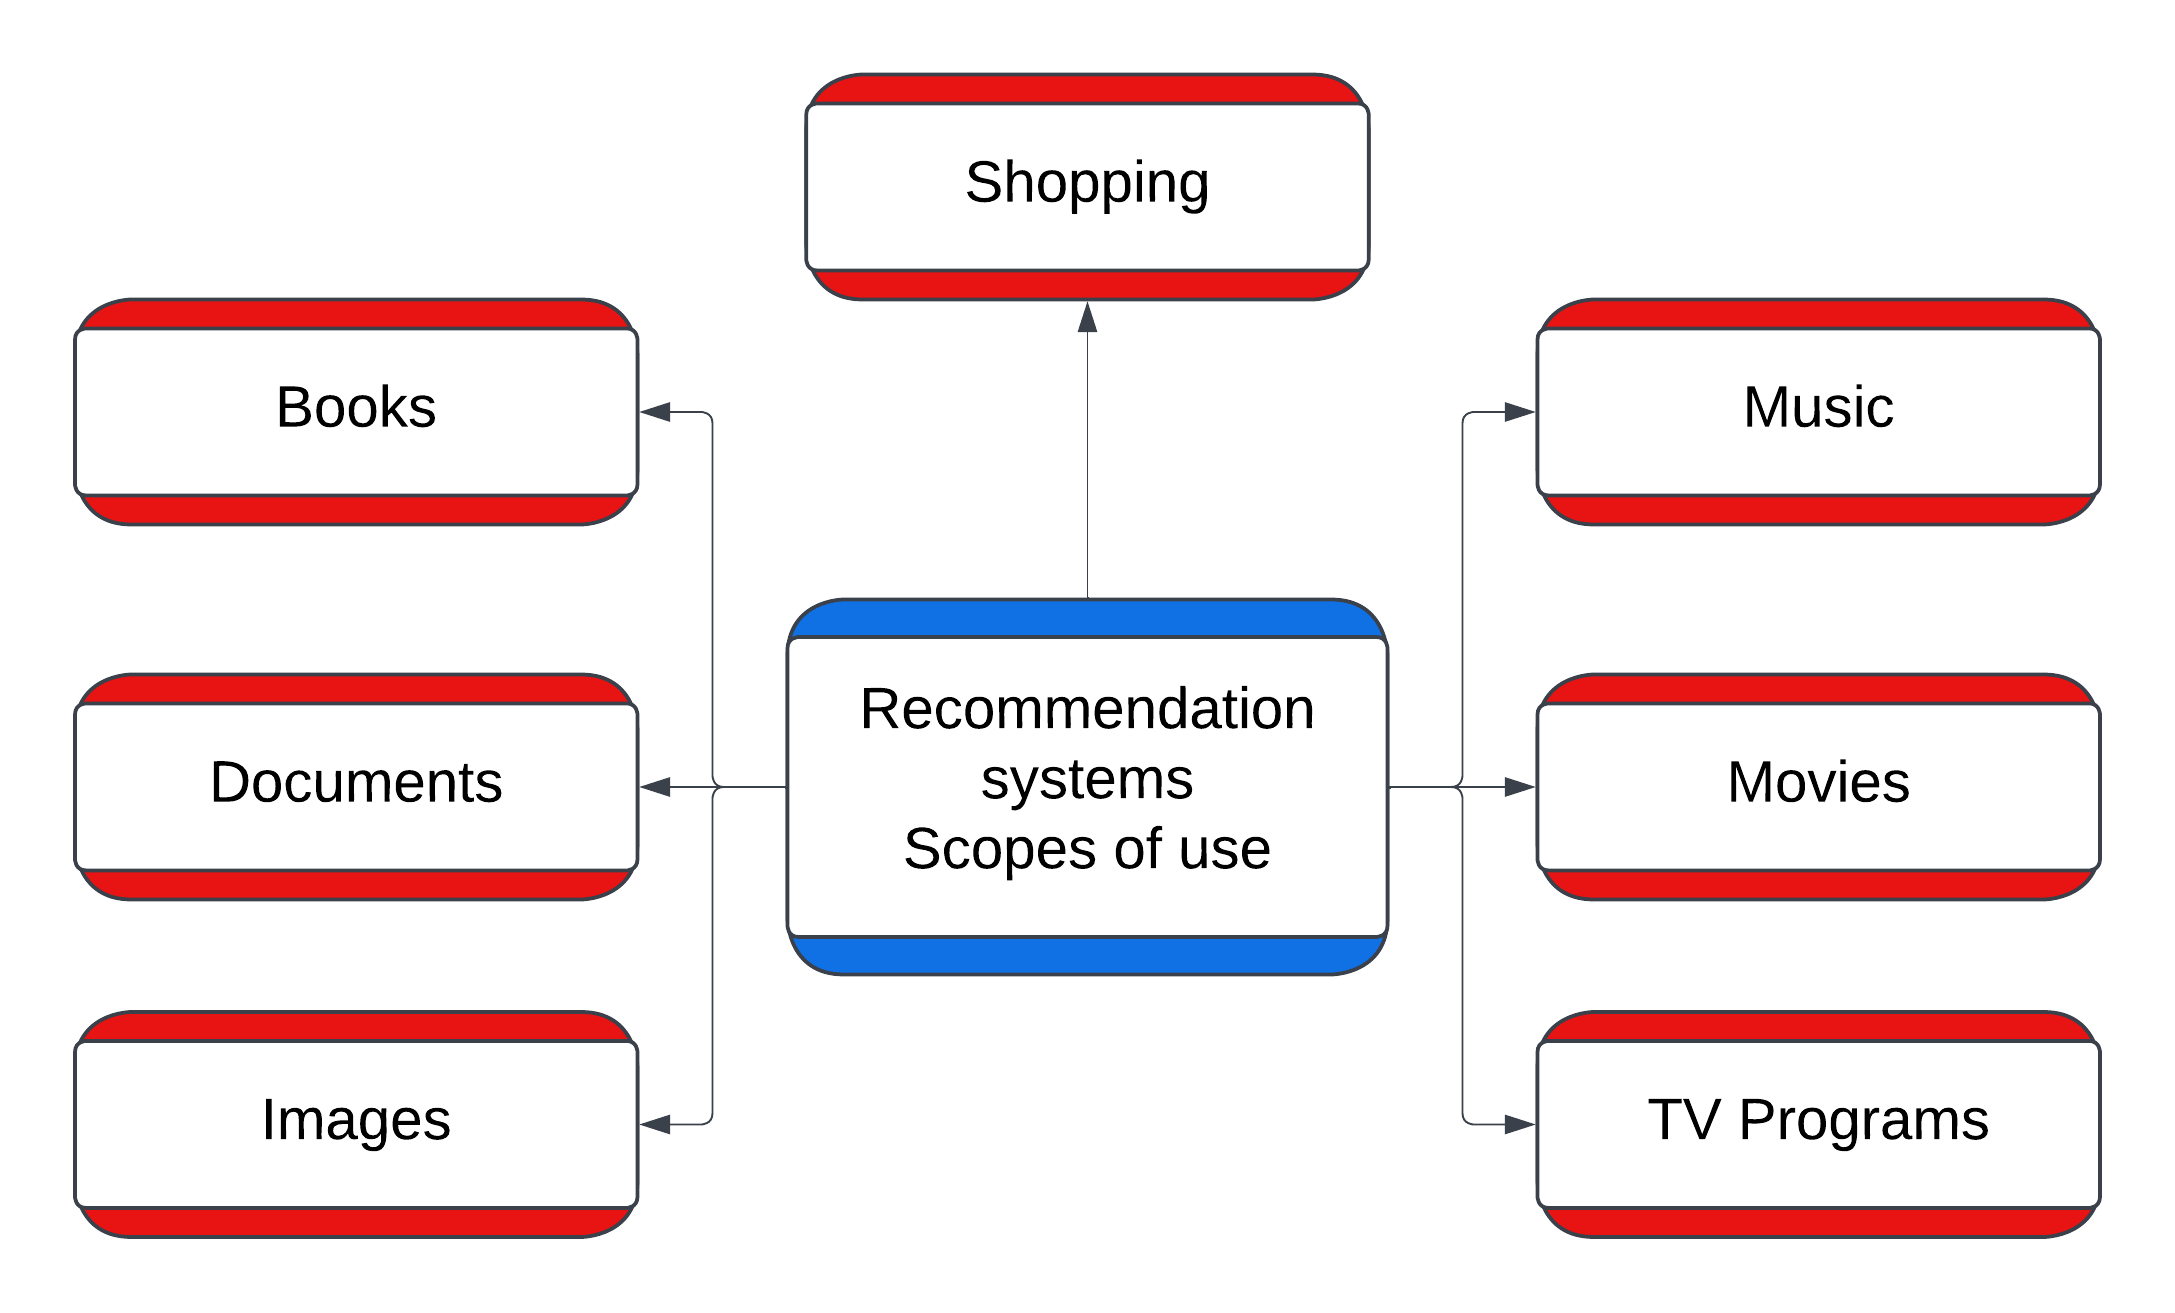
\includegraphics[width=0.8\textwidth]{system_types}

%\end{figure}

\end{center}
Some of the \textbf{greatest}
discoveries in \underline{science} 
were made by \textbf{\textit{accident}}.


% \section{Introduction}

% Motivate the reader and explain what you're going to write about. Introduction mostly of the times doesn't seclude on more than 1 part.

% State explicitly the structure of the article. Here is some example.
% The basic problem that was indicated in the introduction is explained in more detail in the section~\ref{any}.
% Important contexts are given is sections~\ref{important} and~\ref{significant}.
% Concluding notations establishes part~\ref{inference}.



% \section{Some part} \label{any}

% From pic.~\ref{f:rozhod} everything is clear. 

% \begin{figure*}[tbh]
% \centering
% %\includegraphics[scale=1.0]{diagram.pdf}
% Text can also be presented as an image. It will become a marker floating object. After creating the diagram, cancel the sign \texttt{\%} before the command\verb|\includegraphics| denote this row as a comment (also using symbol\texttt{\%}).
% \caption{Choosing argument.}
% \label{f:rozhod}
% \end{figure*}



% \section{Another part} \label{another}

% The main problem is\ldots{} First things first let's look at an explanation (part~\ref{another:any}), and than on another (part~\ref{another:any}).\footnote{Sometimes you might need symbol over a footer too.}

% It can seem like problem doesn't exist\cite{Coplien:MPD}, but it was proved wrong~\cite{Czarnecki:Staged, Czarnecki:Progress}. Nevertheless, even today on the web we come across all kinds of dubious opinions\cite{PLP-Framework}. Important thing can be \emph{emphasized by cursive text}.


% \subsection{Some sort of explanation} \label{another:any}

% Sometimes you need to make a list:

% \begin{itemize}
% \item First thing
% \item Second thing
% 	\begin{itemize}
% 	\item First item
% 	\item Second item
% 	\end{itemize}
% \end{itemize}

% The same list but marked by letters and numbers:

% \begin{enumerate}
% \item First thing
% \item Second thing
% 	\begin{enumerate}
% 	\item First item
% 	\item second item
% 	\end{enumerate}
% \end{enumerate}


% \subsection{Some more explanation} \label{something different:etc.}

% \paragraph{Something very important.}
% Sometimes it is necessary to mark a paragraph with a heading. Text continues straight after the denotation.



% \section{An important part} \label{important}


% \section{}


% \section{Even more significant part} \label{more important}




% \section{Inference} \label{conclusion} % prípadne iný variant názvu



% %\acknowledgement{Ak niekomu chcete poďakovať\ldots}


% % týmto sa generuje zoznam literatúry z obsahu súboru literatura.bib podľa toho, na čo sa v článku odkazujete
% \bibliography{literature}
% \bibliographystyle{alpha} % prípadne alpha, abbrv alebo hociktorý iný

% Sources

%Shcolar - https://link.springer.com/chapter/10.1007/978-981-13-7025-0_34
%Scolar - https://www.sciencedirect.com/science/article/pii/S0957417412002825#f0005 
\end{document}
